\section{Características ARM}

O termo ARM se refere a \emph{Advanced RISC Machine}, ou seja uma arquitetura que usa o conceito conhecido como RISC. RISC, \emph{Reduced Instruction Set Computer}, é uma linha de arquitetura que possui um conjunto simples e pequeno de instruções que levam aproximadamente a mesma quantidade de tempo para serem executadas, permitindo que estes processadores tenham menos transístores do que aqueles projetados na arquitetura convencional. Logo essa abordagem reduz a liberação de calor, o consumo de energia e a quantidade de componentes em um processador.

Segundo  Yiu \cite{ARMGUIDE} a arquitetura dos processadores usados aqui, o Cortex-M3 e Cortex-M4, são ambos as implementações da arquitetura ARMv7-M. Existem diferentes tipos de arquitetura ARM para diferentes tipos de processadores, que ainda podem variar conforme são atualizadas ao longo dos anos. Os detalhes da arquitetura ARMv7-M estão documentados no Manual de Referência, disponível no site da  \href{http://infocenter.arm.com/help/index.jsp}{ARM Limited}.

O Cortex-M3 e Cortex-M4 são essencialmente idênticos em seus aspectos construtivos, de modo que o diagrama de blocos da figura \ref{DiagramaDeBlocosARM}  apresenta uma visão  geral interna adequada tanto do processador Cortex –M4 quanto -M3.

\begin{figure}[h]
	\centering
	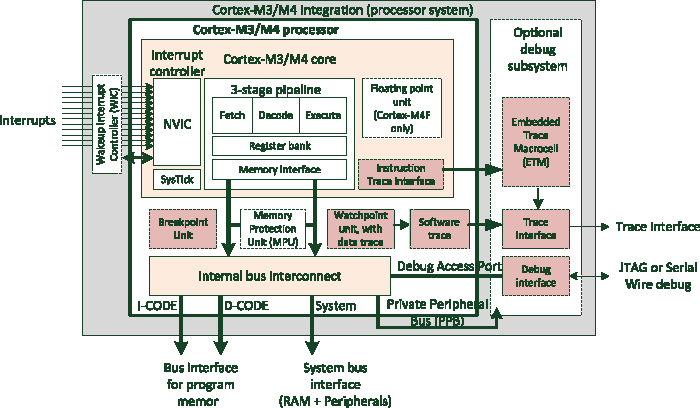
\includegraphics[scale=0.9]{DiagramaDeBlocosARM}
	\caption{Diagrama de Blocos - Processador Cortex-M3 e Cortex-M4 \cite{DATASHEET_TIVA}}
	\label{DiagramaDeBlocosARM}
\end{figure}

Na figura \ref{DiagramaDeBlocosARM} notamos a presença de elementos no processador como:  o controlador de vetores de interrupção, NVIC (\emph{Nested Vectored Interrupt Controller}); o controlador de acionamento de interrupção, WIC (\emph{Wakeup Interrupt Controller}); o temporizador SysTick; a unidade de proteção de memória MPU (\emph{Memory Protection Unit}); e uma unidade de ponto flutuante presente apenas no Cortex –M4. Existe ainda um sistema de debug dentro do processador para realizar depuração de software e um sistema interno de barramentos para transferência de dados entre o núcleo do processador, o sistema de debug e o MPU. 

Os processadores da família Cortex M são de 32 bits, podendo também trabalhar com dados de 8 bits e 16 bits de forma bastante eficiente. Já os processadores Cortex-M3  e Cortex-M4, mesmo sendo da família Cortex M, podem realizar uma série de operações envolvendo dados de 64 bits. Estas operações podem ser realizadas através de um \emph{piperline} de três estágios com uma arquitetura de barramento do tipo \emph{Harvard} permitindo instruções simultâneas de busca e acesso de dados.

Uma das grandes vantagens dos processadores Cortex M é seu baixo consumo de energia. Em especial os processadores Cortex M3 e Cotex M4 podem executar instruções com taxa de $200 mA/MHz$ com alimentação de $1,8 V$. Estes processadores possuem modos de suspensão que tornam possíveis desativar dispositivos de \emph{Clock} para economizar energia, e um \emph{hardware} adicional para despertar o processador dos modos de suspensão.

Devemos salientar aqui que estamos sempre nos referindo a apenas aos processadores, e que este é uma parte constituinte do microcontrolador. De modo que os demais componentes da placa são desenvolvidos pelos diferentes fabricantes. Assim existem vários tipos de microcontroladores com diferentes características de periféricos e recursos, porém a arquitetura empregada nos processadores é a mesma.


\section{Modos de operação ARM Cortex-M4}

O processador Cortex-M4 possui dois estados de operação, como mostrado na figura \ref{fig:modosDeOperacao}, \emph{debug state} e \emph{Thumb state}. O \emph{debug state} ocorre quando o processador é interrompido, por exemplo ao atingir um \emph{breakpoint}, então a execução de instrução é interrompida. Já o \emph{Thumb state} ocorre quando o código do programa está sendo executado. Diferente de outros processadores ARM, o Cortex-M não suporta instruções ARM.

\begin{figure}[H]
	\centering
	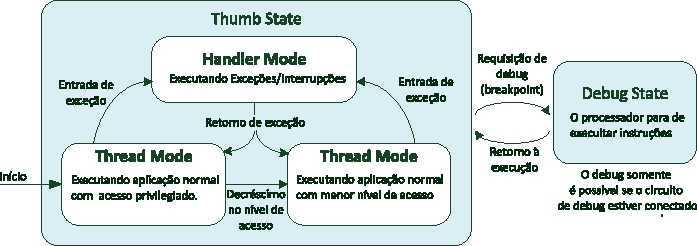
\includegraphics[scale=0.9]{modosDeOperacaoCortex-M4}
	\caption{Modos de Operação \cite{DATASHEET_TIVA}}
	\label{fig:modosDeOperacao}
\end{figure}

No \emph{Thumb state} ainda existem dois modos de operação, que dizem respeito ao nível de privilégio no acesso ao processador. Ao executar uma rotina de tratamento de interrupção o processador entra em um nível de acesso privilegiado, caracterizando o \emph{handler mode}. Durante a execução de uma aplicação normal o processador pode estar tanto em nível de acesso privilegiado quanto em nível menor, sendo chamado de \emph{thread mode}. Isso é controlado por um registrador específico. 

A aplicação pode alterar seu nível de acesso durante o \emph{thread mode}, para um nível menos privilegiado. Porém, para aumentar seu nível de acesso deve haver um mecanismo de exceção/interrupção por parte do processador.  Tais mecanismos de controle de nível de acesso garantem uma maior robustez para o sistema, controlando o acesso à regiões críticas de memória.

\section{Registradores internos}

Para um controle melhor e um processamento de dados maior o Cortex-M4 possui registradores internos ao processador agrupados em um conjunto chamado de \emph{banco de registradores}. Cada instrução enviada ao processador especifica a operação a ser executada, os registradores fonte e se necessário os registradores de destino. A arquitetura ARM é baseada no modelo conhecido como \emph{load/store}, ou seja, para processar um conteúdo que esteja na memória é preciso carregá-lo para um registrador interno e então processá-lo. Se necessário, é preciso armazená-lo de volta na memória.

\begin{figure}[H]
	\centering
	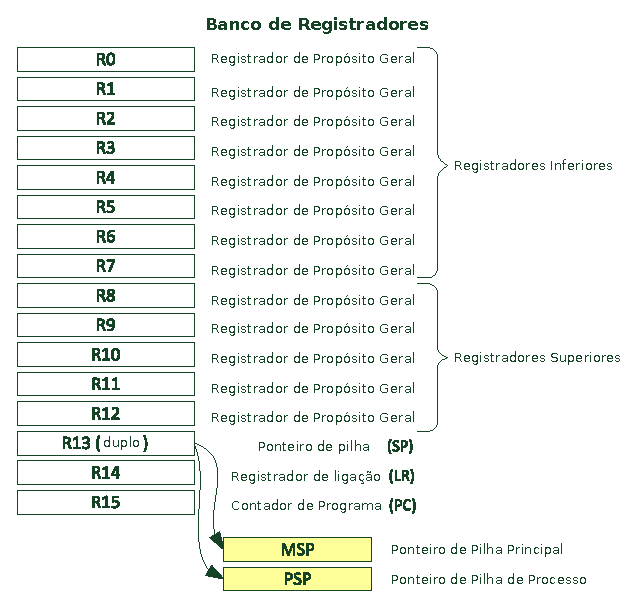
\includegraphics[scale=0.9]{bancoRegistradores}
	\caption{Banco de registradores internos \cite{DATASHEET_TIVA}}
	\label{fig:bancoRegistradores}
\end{figure}

O banco de registradores do Cortex-M4 possui 16 registradores de 32 bits, como mostrado na Figura \ref{fig:bancoRegistradores}. Cada registrador possui seu propósito, como detalhado a seguir:

\begin{description}
\item[R0 - R12: Registradores de Propósito Geral]\hfill \\
Devido ao número limitado no conjunto de instruções, muitas das de 16 bits somente acessam os registradores de R0 à R7, chamados de \emph{registradores inferiores}. De R8 à R9, os \emph{registradores altos}, podem ser usados com as instruções de 32 de bits e alguns com instruções 16 de bits. Os valores iniciais desses registradores são indefinidos.

\item[R13: Ponteiro de Pilha (\emph{Stack Pointer}, SP)]\hfill \\
Usado para acessar a pilha de memória. Fisicamente há dois ponteiros de pilha, o principal (\emph{Main Stack Pointer}, MSP) e o de processo (\emph{Process Stack Pointer}, PSP)). O MSP é o ponteiro padrão, é selecionado após um \emph{reset} do sistema ou quando o processador está em modo de exceção (Handler Mode). Seu valor inicial é o primeiro da memória na sequência de \emph{reset}. Já o PSP é usado durante o Thread Mode, quando as tarefas da aplicação estão rodando, seu valor inicial é desconhecido.

Somente um dos ponteiros de pilha é visível durante a aplicação e os dois bits menos significativos de ambos são sempre nulos. Em aplicações que não fazem uso de um sistema operacional somente o MSP é usado.

\item[R14: Registrador de Ligação (\emph{Link Register}, LR)]\hfill \\
Esse registrador armazena automaticamente o ponto em que uma rotina chama uma sub-rotina. Assim, ao fim da execução dessa sub-rotina, esse valor é carregado para o Contador de Programa e a execução continua de onde tinha anteriormente parado.

Se uma sub-rotina chamar outra sub-rotina, o valor nesse registrador será substituído e o ponto de retorno antigo se perderá, portanto é preciso que esse último valor seja salvo na pilha de memória.

Durante uma rotina de tratamento de exceção, o valor de LR é também sobrescrito mas por um valor de retorno de exceção, usado para disparar o retorno da exceção ao fim da rotina de tratamento.

\item[R15: Contador de Programa (\emph{Program Counter, PC})]\hfill \\
Marca o próximo endereço que deve ser executado na aplicação. Quando este registrador é lido, automaticamente seu valor decrementa de 4 (32 bits), apontando para o próximo endereço da execução. Já quando é feito uma operação de escrita, o programa pula para a posição apontada e passa a executar a aplicação a partir deste novo ponto.

O bit menos significativo do PC indica o tipo de instrução que está sendo executada, '0' para ARM e '1' para Thumb. Portanto no Cortex-M4, tal bit deve ser sempre '1' pois não são suportadas instruções ARM. Este fato deve ser lembrado quando é feita uma operação de escrita sobre o registrador.

\end{description}